% Hausa Med QA -- pilot study manuscript.
%
% Every number comes from % Generated by src/paper.py from results/. Do not edit by hand.
% Regenerate:  python -c "from src import paper, figures as F; paper.write_numbers(F.load())"

\newcommand{\BaselineP}{0.318}
\newcommand{\Chance}{0.25}
\newcommand{\ConsEnLlama}{0.670}
\newcommand{\ConsEnMedGemma}{0.578}
\newcommand{\ConsEnQwen}{0.676}
\newcommand{\ConsGapLlama}{0.460}
\newcommand{\ConsGapMedGemma}{0.170}
\newcommand{\ConsGapQwen}{0.592}
\newcommand{\ConsHaLlama}{0.210}
\newcommand{\ConsHaMedGemma}{0.408}
\newcommand{\ConsHaQwen}{0.084}
\newcommand{\EFormat}{0.04}
\newcommand{\EFormatHi}{0.14}
\newcommand{\EFormatLo}{0.01}
\newcommand{\EFormatN}{2}
\newcommand{\ELocChosen}{10}
\newcommand{\ELocGold}{6}
\newcommand{\ELocStem}{18}
\newcommand{\ENRows}{50}
\newcommand{\EReason}{0.28}
\newcommand{\EReasonHi}{0.42}
\newcommand{\EReasonLo}{0.17}
\newcommand{\EReasonN}{14}
\newcommand{\ETerm}{0.58}
\newcommand{\ETermHi}{0.71}
\newcommand{\ETermLo}{0.44}
\newcommand{\ETermN}{29}
\newcommand{\ETextTotal}{34}
\newcommand{\ETrans}{0.10}
\newcommand{\ETransHi}{0.21}
\newcommand{\ETransLo}{0.04}
\newcommand{\ETransN}{5}
\newcommand{\EUntranslated}{22}
\newcommand{\EnLlama}{0.618}
\newcommand{\EnMedGemma}{0.550}
\newcommand{\EnQwen}{0.526}
\newcommand{\ExclDental}{1318}
\newcommand{\ExclMultiAnswer}{894}
\newcommand{\FallbackItems}{95}
\newcommand{\GapHiLlama}{39.4}
\newcommand{\GapHiMedGemma}{24.4}
\newcommand{\GapHiQwen}{45.4}
\newcommand{\GapLlama}{34.2}
\newcommand{\GapLoLlama}{28.8}
\newcommand{\GapLoMedGemma}{14.4}
\newcommand{\GapLoQwen}{35.2}
\newcommand{\GapMedGemma}{19.4}
\newcommand{\GapQwen}{40.4}
\newcommand{\GateAcc}{0.079}
\newcommand{\GateAccParsed}{0.198}
\newcommand{\GateAccParsedHi}{0.289}
\newcommand{\GateAccParsedLo}{0.131}
\newcommand{\GateItems}{60}
\newcommand{\GateK}{4}
\newcommand{\GateLuck}{1.00}
\newcommand{\GatePairs}{17}
\newcommand{\GateParse}{0.400}
\newcommand{\GateParsedN}{96}
\newcommand{\GateProjected}{122}
\newcommand{\GateSamples}{240}
\newcommand{\GateThreshold}{200}
\newcommand{\GateUnparsedPct}{60.0}
\newcommand{\GateZeroItems}{43}
\newcommand{\GateZeroPct}{71.7}
\newcommand{\HaEnLlama}{0.450}
\newcommand{\HaEnMedGemma}{0.402}
\newcommand{\HaEnQwen}{0.392}
\newcommand{\HaLlama}{0.276}
\newcommand{\HaMedGemma}{0.356}
\newcommand{\HaQwen}{0.122}
\newcommand{\LpHaLlama}{0.274}
\newcommand{\LpHaMedGemma}{0.360}
\newcommand{\LpHaQwen}{0.266}
\newcommand{\MarginLlama}{-4.2}
\newcommand{\MarginMedGemma}{3.8}
\newcommand{\MarginQwen}{-19.6}
\newcommand{\NBelowBaseline}{2}
\newcommand{\NEval}{500}
\newcommand{\NModels}{3}
\newcommand{\ParseEnLlama}{1.00}
\newcommand{\ParseEnMedGemma}{1.00}
\newcommand{\ParseEnQwen}{1.00}
\newcommand{\ParseHaLlama}{1.00}
\newcommand{\ParseHaMedGemma}{1.00}
\newcommand{\ParseHaQwen}{0.47}
\newcommand{\PoolRemaining}{1936}
\newcommand{\PoolStart}{4183}
\newcommand{\RecHiLlama}{0.63}
\newcommand{\RecHiMedGemma}{0.45}
\newcommand{\RecHiQwen}{0.77}
\newcommand{\RecLlama}{0.51}
\newcommand{\RecLoLlama}{0.38}
\newcommand{\RecLoMedGemma}{-0.01}
\newcommand{\RecLoQwen}{0.57}
\newcommand{\RecMedGemma}{0.24}
\newcommand{\RecPLlama}{0.000}
\newcommand{\RecPMedGemma}{0.073}
\newcommand{\RecPQwen}{0.000}
\newcommand{\RecQwen}{0.67}
\newcommand{\SensAN}{499}
\newcommand{\SensAShift}{0.1}
\newcommand{\SensBN}{405}
\newcommand{\SensBShift}{2.8}
\newcommand{\ValAdequacyOne}{4.52}
\newcommand{\ValAdequacyTwo}{4.36}
\newcommand{\ValFlagged}{1}
\newcommand{\ValGeFourOne}{1.00}
\newcommand{\ValGeFourOnePct}{100.0}
\newcommand{\ValGeFourTwo}{0.99}
\newcommand{\ValGeFourTwoPct}{98.7}
\newcommand{\ValKappa}{-0.30}
\newcommand{\ValMinGeFourPct}{98.7}
\newcommand{\ValN}{75}
, generated by src/paper.py from
% results/. Do not type a figure into this file: add it to src/paper.py and use
% the macro, so the text cannot drift from the results.
%
% Compile on Overleaf (or arXiv itself): pdflatex -> bibtex -> pdflatex x2.
% Check macros first:
%   python -c "from src import paper, figures as F; print(paper.check_macros())"
%
% TODO BEFORE SUBMISSION -- these need a human, and are marked \todo{} below:
%   * author names, affiliations, contact
%   * the second rater and second coder, credited with their consent (section 11
%     of the pre-registration commits to this)
%   * related work: this draft sketches the shape, you choose the citations
%   * the H4 section, once notebook 03a has run
\documentclass[11pt,a4paper]{article}

\usepackage[utf8]{inputenc}
\usepackage[T1]{fontenc}
\usepackage{lmodern}
\usepackage[margin=1in]{geometry}
\usepackage{graphicx}
\usepackage{booktabs}
\usepackage{amsmath}
\usepackage{url}
\usepackage[hidelinks]{hyperref}
\usepackage{xcolor}

\newcommand{\todo}[1]{\textcolor{red}{[TODO: #1]}}
% Generated by src/paper.py from results/. Do not edit by hand.
% Regenerate:  python -c "from src import paper, figures as F; paper.write_numbers(F.load())"

\newcommand{\BaselineP}{0.318}
\newcommand{\Chance}{0.25}
\newcommand{\ConsEnLlama}{0.670}
\newcommand{\ConsEnMedGemma}{0.578}
\newcommand{\ConsEnQwen}{0.676}
\newcommand{\ConsGapLlama}{0.460}
\newcommand{\ConsGapMedGemma}{0.170}
\newcommand{\ConsGapQwen}{0.592}
\newcommand{\ConsHaLlama}{0.210}
\newcommand{\ConsHaMedGemma}{0.408}
\newcommand{\ConsHaQwen}{0.084}
\newcommand{\EFormat}{0.04}
\newcommand{\EFormatHi}{0.14}
\newcommand{\EFormatLo}{0.01}
\newcommand{\EFormatN}{2}
\newcommand{\ELocChosen}{10}
\newcommand{\ELocGold}{6}
\newcommand{\ELocStem}{18}
\newcommand{\ENRows}{50}
\newcommand{\EReason}{0.28}
\newcommand{\EReasonHi}{0.42}
\newcommand{\EReasonLo}{0.17}
\newcommand{\EReasonN}{14}
\newcommand{\ETerm}{0.58}
\newcommand{\ETermHi}{0.71}
\newcommand{\ETermLo}{0.44}
\newcommand{\ETermN}{29}
\newcommand{\ETextTotal}{34}
\newcommand{\ETrans}{0.10}
\newcommand{\ETransHi}{0.21}
\newcommand{\ETransLo}{0.04}
\newcommand{\ETransN}{5}
\newcommand{\EUntranslated}{22}
\newcommand{\EnLlama}{0.618}
\newcommand{\EnMedGemma}{0.550}
\newcommand{\EnQwen}{0.526}
\newcommand{\ExclDental}{1318}
\newcommand{\ExclMultiAnswer}{894}
\newcommand{\FallbackItems}{95}
\newcommand{\GapHiLlama}{39.4}
\newcommand{\GapHiMedGemma}{24.4}
\newcommand{\GapHiQwen}{45.4}
\newcommand{\GapLlama}{34.2}
\newcommand{\GapLoLlama}{28.8}
\newcommand{\GapLoMedGemma}{14.4}
\newcommand{\GapLoQwen}{35.2}
\newcommand{\GapMedGemma}{19.4}
\newcommand{\GapQwen}{40.4}
\newcommand{\GateAcc}{0.079}
\newcommand{\GateAccParsed}{0.198}
\newcommand{\GateAccParsedHi}{0.289}
\newcommand{\GateAccParsedLo}{0.131}
\newcommand{\GateItems}{60}
\newcommand{\GateK}{4}
\newcommand{\GateLuck}{1.00}
\newcommand{\GatePairs}{17}
\newcommand{\GateParse}{0.400}
\newcommand{\GateParsedN}{96}
\newcommand{\GateProjected}{122}
\newcommand{\GateSamples}{240}
\newcommand{\GateThreshold}{200}
\newcommand{\GateUnparsedPct}{60.0}
\newcommand{\GateZeroItems}{43}
\newcommand{\GateZeroPct}{71.7}
\newcommand{\HaEnLlama}{0.450}
\newcommand{\HaEnMedGemma}{0.402}
\newcommand{\HaEnQwen}{0.392}
\newcommand{\HaLlama}{0.276}
\newcommand{\HaMedGemma}{0.356}
\newcommand{\HaQwen}{0.122}
\newcommand{\LpHaLlama}{0.274}
\newcommand{\LpHaMedGemma}{0.360}
\newcommand{\LpHaQwen}{0.266}
\newcommand{\MarginLlama}{-4.2}
\newcommand{\MarginMedGemma}{3.8}
\newcommand{\MarginQwen}{-19.6}
\newcommand{\NBelowBaseline}{2}
\newcommand{\NEval}{500}
\newcommand{\NModels}{3}
\newcommand{\ParseEnLlama}{1.00}
\newcommand{\ParseEnMedGemma}{1.00}
\newcommand{\ParseEnQwen}{1.00}
\newcommand{\ParseHaLlama}{1.00}
\newcommand{\ParseHaMedGemma}{1.00}
\newcommand{\ParseHaQwen}{0.47}
\newcommand{\PoolRemaining}{1936}
\newcommand{\PoolStart}{4183}
\newcommand{\RecHiLlama}{0.63}
\newcommand{\RecHiMedGemma}{0.45}
\newcommand{\RecHiQwen}{0.77}
\newcommand{\RecLlama}{0.51}
\newcommand{\RecLoLlama}{0.38}
\newcommand{\RecLoMedGemma}{-0.01}
\newcommand{\RecLoQwen}{0.57}
\newcommand{\RecMedGemma}{0.24}
\newcommand{\RecPLlama}{0.000}
\newcommand{\RecPMedGemma}{0.073}
\newcommand{\RecPQwen}{0.000}
\newcommand{\RecQwen}{0.67}
\newcommand{\SensAN}{499}
\newcommand{\SensAShift}{0.1}
\newcommand{\SensBN}{405}
\newcommand{\SensBShift}{2.8}
\newcommand{\ValAdequacyOne}{4.52}
\newcommand{\ValAdequacyTwo}{4.36}
\newcommand{\ValFlagged}{1}
\newcommand{\ValGeFourOne}{1.00}
\newcommand{\ValGeFourOnePct}{100.0}
\newcommand{\ValGeFourTwo}{0.99}
\newcommand{\ValGeFourTwoPct}{98.7}
\newcommand{\ValKappa}{-0.30}
\newcommand{\ValMinGeFourPct}{98.7}
\newcommand{\ValN}{75}


\title{Medical question answering collapses in Hausa:\\
a pre-registered pilot on three small open models}

\author{\todo{authors, affiliations, contact}}
\date{\today}

\begin{document}
\maketitle

\begin{abstract}
We ask how much accuracy and answer stability small open language models lose
when medical multiple-choice questions are posed in Hausa rather than English.
On a paired English--Hausa set of \NEval{} MedMCQA items, three instruction-tuned
models of 3--4B parameters lose between \GapMedGemma{} and \GapQwen{} percentage
points of accuracy, every gap significant after Holm correction. The more
useful finding is the reference point: a trivial baseline that reads nothing and
always answers the most frequent letter scores \BaselineP{}, and two of the three
models fall at or below it in Hausa. Back-translating the Hausa items into
English recovers roughly half the gap for two models but not demonstrably for
the third, so the deficit is substantially, though not wholly, a matter of the
language of presentation. Answers are also far less stable: agreement under
option reordering falls by \ConsGapQwen{} for the worst model. An exploratory
error analysis of \ENRows{} discordant items attributes most of the damage to
medical vocabulary lost in translation (\ETerm{}, 95\% CI \ETermLo{}--\ETermHi{}),
usually in the question stem. All hypotheses, thresholds and decision rules were
registered before any model was run, and all deviations are logged.
\end{abstract}

\section{Introduction}

\todo{Two or three paragraphs. The shape:}
\begin{itemize}
  \item Hausa has 50--80 million speakers and almost no medical NLP evaluation.
  \item Small open models are the ones that can plausibly be deployed in
        low-resource clinical settings -- they fit on commodity hardware -- so
        their behaviour in the target language is the practical question.
  \item Benchmarks report English numbers. We ask what is left in Hausa, and we
        pre-register the question so the answer is not chosen after the fact.
  \item Contributions: (i) a paired English--Hausa medical MCQ set with human
        validation; (ii) a pre-registered evaluation of three models with
        decision rules fixed in advance; (iii) the observation that the usual
        way of reporting such gaps -- a percentage drop -- hides that the
        post-drop score is at or below a trivial baseline.
\end{itemize}

\section{Related work}

\todo{Choose citations. The three strands: multilingual medical QA benchmarks
and MedMCQA itself; evaluation of LLMs on African languages, AfriMed-QA and
related resources; and position/format sensitivity in multiple-choice
evaluation, which is why we report a majority-letter baseline and measure
consistency under option reordering at all.}

\section{Data}

We sample from the MedMCQA validation split, whose labels are public. Of
\PoolStart{} items we remove Dental (\ExclDental{} items, outside this study's
general-health motivation and about 30\% of the split), multi-answer items
(\ExclMultiAnswer{}), items whose options are position-dependent (``all of the
above'' and similar), and items that require an image the model cannot see,
leaving \PoolRemaining{}. From these we draw \NEval{} evaluation items stratified
by subject with a fixed seed. MedMCQA contains a scraping artifact in which the
letter pair ``rt'' is deleted from many words (``aery'' for artery); we repair it
with a fixed rule list before filtering.

Hausa versions are produced with NLLB-200-3.3B. Segment-level quality is
estimated by round-trip chrF1 with a second, distilled model, and flagged
segments are reviewed by a native speaker who records one of \emph{keep},
\emph{english} (use the English term, as is common for medical vocabulary in
Hausa) or \emph{edit}. \FallbackItems{} items retain at least one English option
after review; a pre-registered sensitivity analysis excludes them.

\paragraph{Human validation.}
Two native speakers independently rated 75 items for adequacy on a 1--5 scale.
Mean adequacy was \ValAdequacyOne{} and \ValAdequacyTwo{}, with \ValGeFourOne{}
and \ValGeFourTwo{} of items rated 4 or better, and no medical-term errors
marked by either rater. Quadratic-weighted $\kappa$ is \ValKappa{}: ratings
concentrate at 4--5, where $\kappa$ is unstable, so we report it as computed and
rely on the agreement that matters -- both raters judged \ValGeFourTwo{} or more
of the items acceptable. \ValFlagged{} item was flagged by either rater.
Both raters reported checking question stems closely and options less closely,
so this validates stem quality better than option quality; we return to this in
the limitations.

\paragraph{Licensing.}
MedMCQA carries two different licences from its own publishers: the source
project is MIT, while the Hugging Face distribution's metadata says
\texttt{apache-2.0} and its licensing section is an unfilled placeholder. Both
permit redistribution of derived text with attribution. The binding constraint
is neither: NLLB-200-3.3B is CC-BY-NC-4.0, so the released Hausa text is
non-commercial only.

\section{Method}

\paragraph{Pre-registration.}
Hypotheses H1--H4, their thresholds and their decision rules were frozen before
any model was run, and are in the repository along with every deviation. Six
deviations are logged; the two that affect the numbers below are an
assistant-turn prefill (the answer turn begins with ``Answer:'' / ``Amsa:'', so
the model's first tokens are the letter) and a secondary letter-probability
scoring rule reported alongside the primary parsed one.

\paragraph{Models and conditions.}
Llama-3.2-3B-Instruct, Qwen2.5-3B-Instruct and MedGemma-4B-IT, all bf16. Each
item is presented in English and in Hausa under a fixed zero-shot template, in
the canonical option order and in two seeded reorderings, plus a
back-translated-to-English condition for H2.

\paragraph{Statistics.}
Paired comparisons use an exact McNemar test with Holm correction across the
three models, and 95\% confidence intervals from a paired bootstrap with 10{,}000
resamples. Consistency (H3) is the proportion of items answered identically
across all three option orders.

\paragraph{The baseline that matters.}
Gold answers are not uniformly distributed over A--D, so we report what a model
scores by reading nothing and always answering the most frequent letter:
\BaselineP{} in the canonical order, against \Chance{} for chance. Every accuracy
below should be read against it.

\section{Results}

\begin{figure}[t]
  \centering
  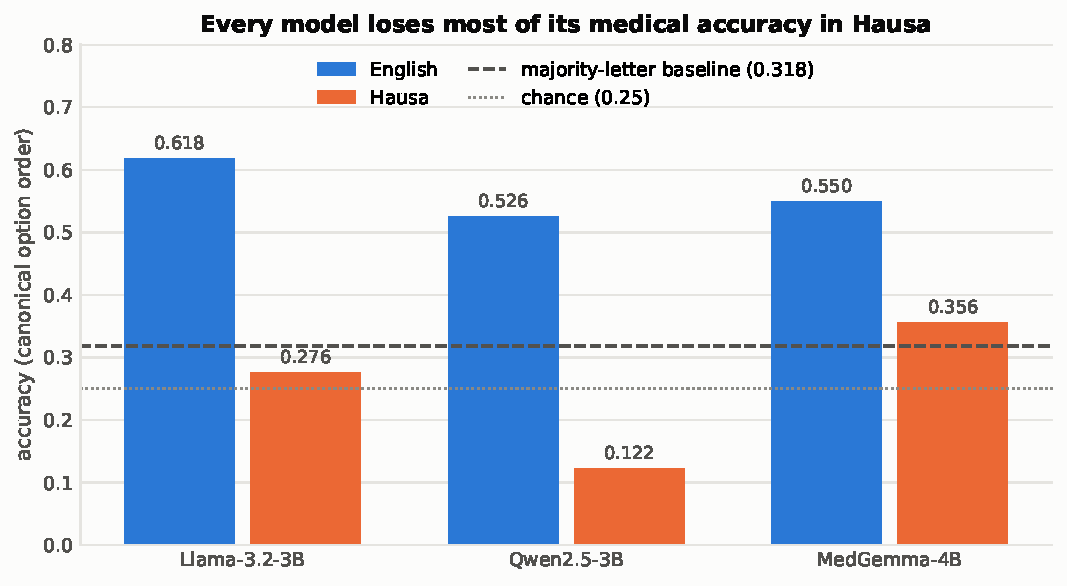
\includegraphics[width=\linewidth]{../results/figures/fig1_accuracy.pdf}
  \caption{English and Hausa accuracy for each model, against the
  majority-letter baseline (\BaselineP{}) and chance. Two of the three models
  fall at or below the baseline in Hausa.}
  \label{fig:accuracy}
\end{figure}

\paragraph{H1: the gap.}
All three models lose a large fraction of their accuracy
(Figure~\ref{fig:accuracy}). Llama falls from \EnLlama{} to \HaLlama{}
(\GapLlama{} pp, 95\% CI \GapLoLlama{}--\GapHiLlama{}), Qwen from \EnQwen{} to
\HaQwen{} (\GapQwen{} pp, \GapLoQwen{}--\GapHiQwen{}), and MedGemma from
\EnMedGemma{} to \HaMedGemma{} (\GapMedGemma{} pp,
\GapLoMedGemma{}--\GapHiMedGemma{}). All three are significant after Holm
correction.

\paragraph{The gap is not the headline.}
Llama's Hausa accuracy (\HaLlama{}) and Qwen's (\HaQwen{}) are at or below the
\BaselineP{} majority-letter baseline. Only MedGemma (\HaMedGemma{}) remains
above it, by under four points. Reporting these systems as retaining ``some''
medical ability in Hausa would be an artifact of comparing against chance rather
than against the strongest trivial strategy available.

\begin{figure}[t]
  \centering
  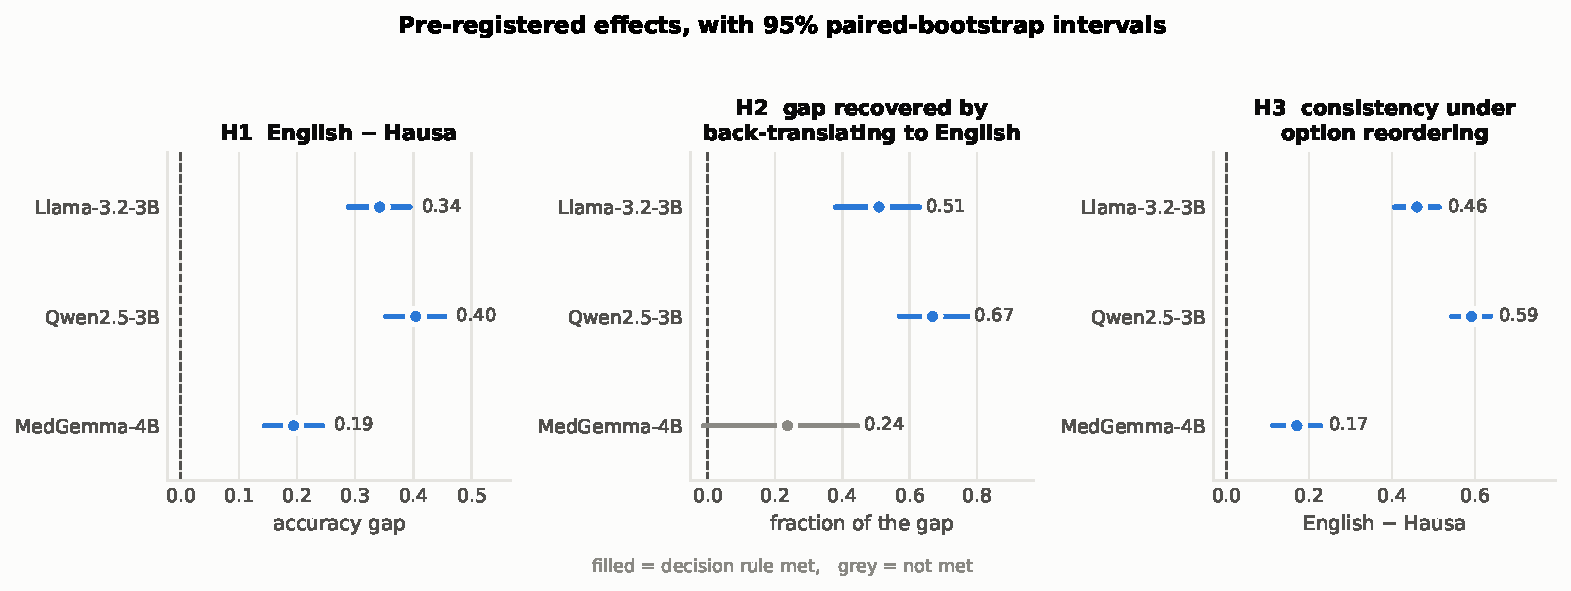
\includegraphics[width=\linewidth]{../results/figures/fig2_effects.pdf}
  \caption{The three pre-registered effects with 95\% paired-bootstrap
  intervals. Grey marks the one decision rule of nine that is not met.}
  \label{fig:effects}
\end{figure}

\paragraph{H2: back-translation.}
Translating the Hausa items back into English and re-asking recovers
\RecLlama{} of Llama's gap (95\% CI \RecLoLlama{}--\RecHiLlama{}) and \RecQwen{}
of Qwen's (\RecLoQwen{}--\RecHiQwen{}), but only \RecMedGemma{} of MedGemma's,
with an interval spanning zero (\RecLoMedGemma{}--\RecHiMedGemma{},
$p=\RecPMedGemma{}$). H2 is therefore supported for two models and not for the
third. Where it holds, much of the deficit travels with the language of
presentation rather than with the medical content.

\paragraph{H3: stability.}
Agreement across the three option orders falls from \ConsEnLlama{} to
\ConsHaLlama{} for Llama, \ConsEnQwen{} to \ConsHaQwen{} for Qwen, and
\ConsEnMedGemma{} to \ConsHaMedGemma{} for MedGemma. Supported for all three.
A Hausa answer is not only likelier to be wrong; it is likelier to change when
the options are shuffled.

\begin{figure}[t]
  \centering
  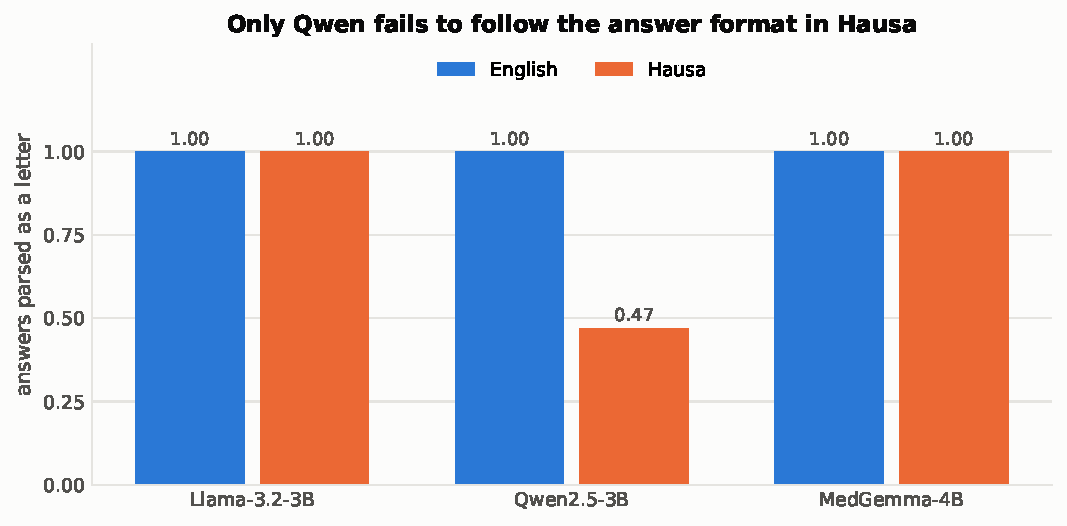
\includegraphics[width=\linewidth]{../results/figures/fig3_parse_rate.pdf}
  \caption{Proportion of answers that could be parsed as a letter. Qwen is the
  exception, and its Hausa deficit is partly a format-following failure.}
  \label{fig:parse}
\end{figure}

\paragraph{Format following, and what the scoring rule carries.}
Llama and MedGemma emit a parseable letter for every Hausa item. Qwen parses
only \ParseHaQwen{} of its Hausa answers against \ParseEnQwen{} in English
(Figure~\ref{fig:parse}). Scoring the identical outputs by the probability of
each letter token rather than by parsing the text moves Qwen from \HaQwen{} to
\LpHaQwen{}, while Llama (\HaLlama{} to \LpHaLlama{}) and MedGemma
(\HaMedGemma{} to \LpHaMedGemma{}) barely move. Reporting only the parsed rule
overstates Qwen's deficit; reporting only letter probability hides a real
failure to follow instructions in Hausa. We report both.

\paragraph{Sensitivity.}
H1 is unchanged when items flagged by either rater are dropped, and when items
retaining an English option are dropped.

\begin{figure}[t]
  \centering
  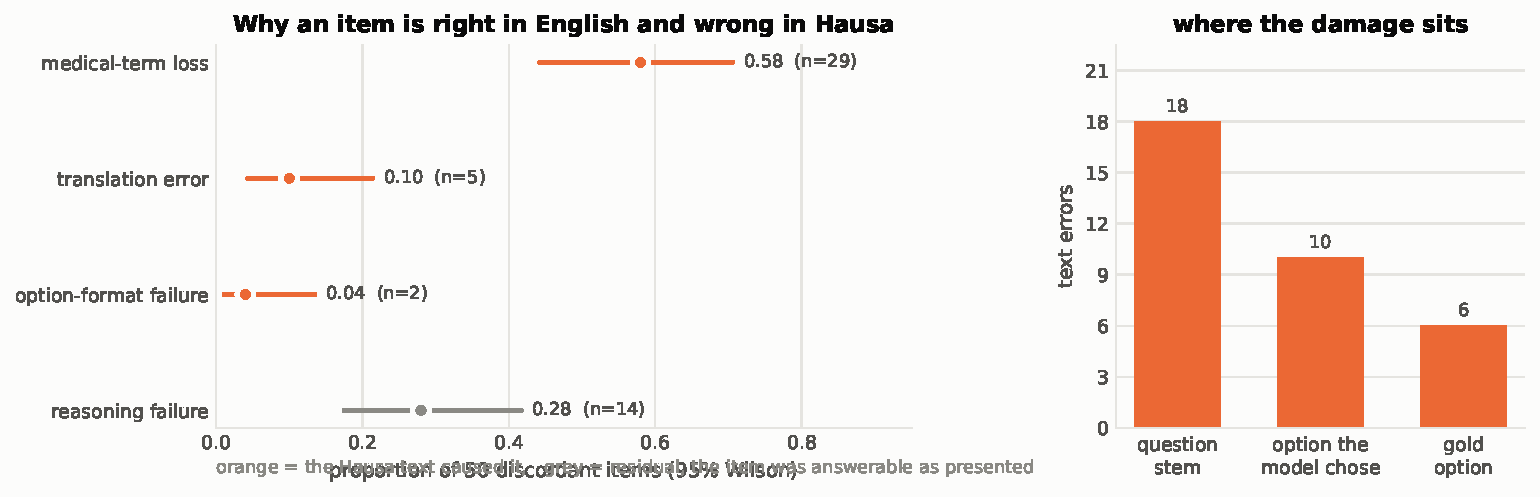
\includegraphics[width=\linewidth]{../results/figures/fig5_e1_errors.pdf}
  \caption{Exploratory error analysis of \ENRows{} items answered correctly in
  English and wrongly in Hausa.}
  \label{fig:errors}
\end{figure}

\paragraph{Exploratory: why items fail.}
We coded \ENRows{} discordant items -- correct in English, wrong in Hausa --
into four categories fixed in advance, under a written codebook with two
machine-enforced consistency rules: a coded segment's Hausa must differ from its
English, and a term or translation error must sit in the question stem, the gold
option or the option the model chose. Medical-term loss accounts for \ETerm{}
(95\% CI \ETermLo{}--\ETermHi{}, $n=\ETermN{}$), residual reasoning failure for
\EReason{}, translation error for \ETrans{} and option-format failure for
\EFormat{}. Of the \ETextTotal{} text errors, \ELocStem{} sit on the question
stem, \ELocChosen{} on the option the model chose and \ELocGold{} on the gold
option. Separately, \EUntranslated{} of the \ENRows{} items carry at least one
option whose Hausa is identical to its English -- untranslated medical
vocabulary, recorded as a descriptive covariate rather than as damage, since the
model sees the same string either way.

This analysis is exploratory, with no hypothesis attached. One coder coded all
items and a second native speaker verified that coding; it is not independent
double coding, and we therefore report no $\kappa$.

\section{H4: can self-generated preference pairs close the gap?}

\todo{Fill in once notebook 03a (the pilot gate) has run. If the gate says
stop, report H4 as not run with the gate as the stated reason and
results/h4\_pilot\_gate.json as the evidence -- that is a legitimate outcome and
was planned for. Note either way: the pre-registered minimum gain is +3 pp on a
base of \HaLlama{}, which reaches 0.306 -- still below the \BaselineP{}
baseline.}

\section{Limitations}

\paragraph{The Hausa set is machine-translated.}
This is the central caveat and it cuts in a specific direction. Our own error
analysis attributes most discordance to the translation rather than to the
model. The measured gap is therefore best read as \emph{the gap a Hausa speaker
would encounter using these models through the best freely available
translation} -- which is the practically relevant quantity -- and not as a clean
measure of multilingual medical reasoning. The human validation subset bounds how
much is translation noise, and both sensitivity analyses leave H1 unchanged.

\paragraph{Option quality is less well validated than stem quality.}
Both raters reported checking stems closely and options less closely.

\paragraph{Scale.}
\NEval{} items, three models of 3--4B parameters, one language. This is a pilot
and is reported as one.

\paragraph{The error analysis is single-coder.}
With a verification pass, under a written codebook with enforced rules, but not
independently double-coded.

\section{Conclusion}

Posed in Hausa, three small open medical-capable models lose most of their
accuracy and much of their stability, and two of the three end up at or below a
baseline that reads nothing at all. The failure is concentrated in medical
vocabulary, mostly in the question stem, and is largely recoverable by
translating back into English -- which suggests the bottleneck for these models
is the language of presentation more than the medicine. We release the paired
set, the human annotation sheets, the pre-registration and every deviation.

\section*{Acknowledgements}
\todo{Credit the second rater and the second coder by name, with their consent
-- section 11 of the pre-registration commits to this.}

\section*{Data and code availability}
Code, pre-registration, deviation log, human annotation sheets and all result
files: \url{https://github.com/avvas200/hausa-med-qa}. The derived Hausa text is
CC-BY-NC-4.0, inherited from NLLB-200.

\bibliographystyle{plain}
\bibliography{refs}

\end{document}
